\documentclass{sig-alternate}
\usepackage{graphicx}
\usepackage{wrapfig,url}
\newcounter{over}
\newcounter{max}
\newcommand{\fred}[2]{\setcounter{over}{#2}\addtocounter{over}{#1}}
\newcommand{\boxplot}[5]{%
\scalebox{0.5}{\textcolor{white}{\setcounter{max}{#4}\addtocounter{max}{#5}\fred{#4}{-#2}}%
\begin{picture}(100,10)%
\put(0,0){\line(0,1){8}}%
\put(100,0){\line(0,1){8}}%
%\put(#1,4){\circle*{1}}%
%\put(\themax,4){\circle*{1}}%
\put(#2,4){\line(1,0){\theover}}%
\put(#3,4){\circle*{8}}%
%\put(#4,4){\line(1,0){#5}}%
\put(50,0){\line(0,1){8}}%
\end{picture}}
} 
\usepackage{eso-pic}
\usepackage{color}
\usepackage{type1cm}
%\makeatletter
%  \AddToShipoutPicture{%
%    \setlength{\@tempdimb}{.5\paperwidth}%
%    \setlength{\@tempdimc}{.5\paperheight}%
%    \setlength{\unitlength}{1pt}%
%      \makebox(600,900){\rotatebox{45}{\textcolor[gray]{0.80}{\fontsize{5cm}{5cm}\selectfont{Draft v5}}}}}
%\makeatother
%
\newenvironment{smallitem}
 {\setlength{\topsep}{0pt}
  \setlength{\partopsep}{0pt}
  \setlength{\parskip}{0pt}
  \begin{itemize}
   \setlength{\leftmargin}{.2in}
  \setlength{\parsep}{0pt}
  \setlength{\parskip}{0pt}
  \setlength{\itemsep}{0pt}}
 {\end{itemize}}
\newenvironment{smallenum}
 {\setlength{\topsep}{0pt}
  \setlength{\partopsep}{0pt}
  \setlength{\parskip}{0pt}
  \begin{enumerate}
  \setlength{\leftmargin}{.2in}
  \setlength{\parsep}{0pt}
  \setlength{\parskip}{0pt}
  \setlength{\itemsep}{0pt}}
 {\end{enumerate}}

 \newcommand{\bd}{\begin{description}}
\newcommand{\ed}{\end{description}}
 \newcommand{\bi}{\begin{smallitem}}
\newcommand{\ei}{\end{smallitem}}
 \newcommand{\be}{\begin{smallenum}}
\newcommand{\ee}{\end{smallenum}}
\newcommand{\fig}[1]{Figure~\ref{fig:#1}}
\newcommand{\eq}[1]{Equation~\ref{eq:#1}}
\newcommand{\tion}[1]{\S\ref{sec:#1}}

%\usepackage{times}
\usepackage{alltt}
\usepackage{url}
% IEEE Computer Society needs nocompress option
% requires cite.sty v4.0 or later (November 2003)
\usepackage{cite}
% normal IEEE
 % \usepackage{cite}

% correct bad hyphenation here
\hyphenation{op-tical net-works semi-conduc-tor}


\pdfpagewidth=8.5in
\pdfpageheight=11in
\begin{document}

%\conferenceinfo{PROMISE'09,} {May 18--19, 2009, Vancouver, Canada} 
\conferenceinfo{~} {~} 

\CopyrightYear{2009}

\crdata{978-1-60558-036-4/08/05}


\title{Simulating the Senate with Intelligent Agents}

\numberofauthors{1}
\author{
\alignauthor Gregory Gay, Tim Menzies
\\
       \affaddr{CS\& EE, WVU, Morgantown, WVU}\\
       \email{greg@greggay.com, tim@menzies.us}
}
%
\date{2 November 2009}

\maketitle
\begin{abstract}
In this research, we model the United States Senate as an intelligent agent system where each Senator is an 
independent agent. 
This is an interesting domain because it provides a space where one-hundred independent 
agents are selfishly trying to complete their goal of passing a bill. However, they must rely on the other agents for support. This 
presents numerous opportunities for observing interesting behavior patterns. 
This research also has the goal of making them act intelligently. To accomplish this, we have implimented a 
treatment learning algorithm called {\em KEYS2}.
\end{abstract}
\category{i.5}{learning}{machine learning}
\keywords{intelligent agents, modeling, simulation}

\section{Introduction}

Intelligent agent systems have become a major topic over the past decade. In these systems, artificial intelligence constructs
attempt to independently solve a series of problems or work within a virtual environment. These agents act without interaction 
from the user and decide on courses of action based on available skills and a derived world view. 

Some of these agent systems are {\em deliberative}. That is, they contain sophisticated theorem-proving algorithms and fleshed-out plan
libraries. These agents tend to be slower, but take more intelligent actions. They are capable of solving greater problems. Other agents are
{\em reactive}. They take actions based on a hierarchy of behaviors where higher actions require more thought. These agents are able to
quickly react to environmental stimuli that would stump deliberative agents. However, they tend to be unable to solve the same kinds of
higher-level issues. 

This research models an interesting domain, the United States Senate. In the Senate, one-hundred elected officials compete, compromise, and
form alliances in order to pass new legislature. This is an interesting domain because it provides a space where one-hundred independent 
agents are selfishly trying to complete their goal of passing a bill. However, they must rely on the other agents for support. This 
presents numerous opportunities for observing interesting behavior patterns. 

In addition to modelling the Senate, this research has the goal of making them act {\em intelligently}. To accomplish this, a 
treatment learning algorithm called {\em KEYS2} is used. This algorithm exploits the key variables within a model and biases actions
that it feels will lead to improved scores (we score based on the average support value that a bill has when it passes). We observe the effects
of this learner over several rounds of feedback.

\section{The Domain}

The intention of this system is to model the United States Senate, the upper house of the legislative branch of the United States government. As established in Article One of the US Constitution ~\cite{const}, the Senate will be made up of one-hundred voting members. Unlike the House of Representatives, which determines membership percentages by state population, each state may only select two senators. Although it is not technically within the scope of this model, it should be noted that the Senate has several powers not allotted to the House of Representatives including the ability to negotiate treaties, to impeach high officials, and to vote on the appointment of certain positions.

In Federalist No. 62, James Madison stated that the "senatorial trust" calls for a "greater extent of information and stability of character." ~\cite{mad62} Thus, the qualifications for becoming a senator are stricter than those of other legislative bodies. All senators must meet the following three requirements: 
\bi
\item Each senator must be at least 30 years old;
\item Must have been a citizen of the United States for at least the past nine years;
\item Must be (at the time of the election) an inhabitant of the state that they seek to represent. 
\ei

Although they were originally selected by state legislatures and not the common population, the ratification of the 17th amendment in 1913 standardized popular election of senators. Senators serve terms of six years each, and may be reelected an unlimited number of times. The seats are staggered such that one third of the senators are up for election every two years. This practices is done to ensure that both seats for a state are not up for contest at the same time. 

Senators may come from any political party, but are likely to belong to either the Republican or Democratic parties. The party with the majority of seats is given certain special positions such as the president pro tempore and the committee chairmen. If neither party has a majority, the party that the Vice President of the United States belongs to becomes the majority party. This simulation decides what party senators belong to stochastically. The real senate is currently made up of fifty-eight Democrats, forty Republicans, one Independent (who sits with the Democrats), and one empty seat (vacated by the death of Senator Ted Kennedy of Massachusetts).

Because very little would be accomplished if every matter required the consent of the entire floor, the United States Senate conducts much of its business through committees and subcommittees. All bills must be reviewed by the appropriate committee before they may be proposed to the Senate as a whole. Membership is determined by the Senate, with senators being given their choice of committees by seniority. Each party is allocated seats on committees in proportion to their overall percentage of floor seats. There are sixteen standing committees:
\bi
\item Agriculture, Nutrition, and Forestry 
\item Appropriations 
\item Armed Services
\item Banking, Housing, and Urban Affairs
\item Budget
\item Commerce, Science, and Transportation
\item Energy and Natural Resources
\item Environment and Public Works
\item Finance
\item Foreign Relations
\item Health, Education, Labor, and Pensions
\item Homeland Security and Governmental Affairs
\item Judiciary
\item Rules and Administration
\item Small Business and Entrepreneurship 
\item Veterans' Affairs 
\ei
The Senate also utilizes multiple subcommittees and non-standing committees, but they are not modeled within this simulation. 

Why model the Senate? The Senate provides us with a discrete group of fascinating agents, all working towards both common and competing goals. Each senator wants to discuss certain issues and pass their own bills, and each political party is working towards what they see as a {\em greater good}. Although each party's goals may run counter to those of the other party, neither has enough of a majority to do any business without help from the other. Therefore, modeling the Senate gives us a collection of competing agents that must be convinced to put aside their own selfish goals temporarily in exchange for help later. While some agent architectures model communities of agents working together, the point of this system is to model a community of agents that must work together despite not neccesarly liking each other. 

\subsection{Domain Compromises}

Because of the limited time allowed to model this domain, and in order to develop a working system, several simplifications have been made. This list is not complete, but these are the major compromises and changes made:
\bi
\item Senators are assigned a party randomly, and the available parties are limited to Democrat and Republican.
\item Senators are assigned a committee randomly. 
\item Committee membership is not controlled by the simulation. Committees are not checked for party composition or number of members. 
\item Senate procedure is simplified, and in some cases, ignored. 
\item Every senator is trying to pass a bill. Therefore, this model is likely to pass many more bills than the real Senate could pass in a single day. 
\item The rules and procedure controlling filibusters have been simplified. 
\item While a senator may propose a bill to the floor only twice per day (like in the real Senate), they may propose a bill to their committee any number of times until is passes. 
\item Committees are implemented, but subcommittees and the special committees do not exist within the simulation.
\item No special positions have been implemented. 
\item There is no tie-breaking mechanism. 
\item All polls require a three/fifths majority to pass. 
\ei

\section{Agent Theory}

\begin{figure}[!t]
\begin{center}
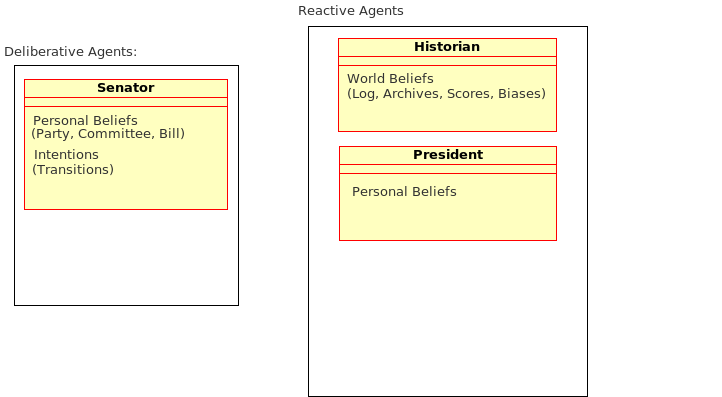
\includegraphics[width=4.5in]{actory2.png}
\end{center}
\caption{Actors as representations of agent theory}
\label{fig:actory2}
\end{figure}

Carl Hewitt remarked in a keynote that the question of what, exactly, 
an agent
is can be as embarrassing a question for the agent-oriented software
development community as the question of what inteligence can be for
the artificial intelligence community. There are
roughly as many definititions as there are researchers. For the
purposes of this work, however, we will default to the definitions 
provided by Michael Woolrdige~\cite{woolridge}. Specifically, {\em agents} can be defined in terms of {\em weak agency} and {\em strong agency}.

Weak Agents are a general type of agent that satisfies the following 
minimal properties: 
\bi
\item Autonomy: The agents operate without direct human intervention and have some control over their actions;
\item Social Ability: Agents can interact with other agents and 
objects within their domain;
\item Reactivity: Agents have knowledge of their environments and can
respond to changes or stimuli from it;
\item Pro-activeness: Agents are able to take actions towards some goal.
\ei 
This weak notion of agency has found wide-use, likely because it is 
a natural extension of the object-oriented software development
paradigm~\cite{Agha86, Agha93}. Many self-contained
processes can satisfy the requirements for weak agency. It can be argued
that such concepts as a Unix software process are weak agents. 

When explaining human behavior, it can be useful to evaluate events 
through the attribution of attitudes - things like believing, wanting,
hoping, fearing, and expecting. These attitudes are called {\em
intentional notions}. A philosopher, Daniel Dennett ~\cite{dennett87}
described intentional systems as those "whose behavious can be predicted
by the method of attributing beliefs, desires, and rational acumen." 
Thus, the difference between weak agents and {\em strong agents} is that
these "strong" agents have explicit notions of beliefs, desires, and
intentions. Strong agents have, and act upon, these intentional notions:
\bi
\item Beliefs: Beliefs represents an agent's view of their domain. 
Thay are a series of facts or variables, and their known values.
They can change over time, certain beliefs can
be forgotten, and new beliefs can be learned. 
\item Desires: These are the goals of an agent. An agent needs to be
pro-actively working towards some sort of goal, even if it is a vague
one like "run until the system shuts down."
\item Intentions: The intentions are the actions that an agent can take
towards completing a goal.  
\ei

When describing agents, the specific software implementation is often
either {\em deliberative}, {\em reactive}, or some hybrid of the two. 
Deliberative agents~\cite{genesereth87} are those that contain an explicitly represented 
model of the world where decisions are guided by some logical reasoning
process. These agents often have explicit notions of beliefs, desires, and
intentions and some sort of theorem proving algorithm to decide which
intentions to follow. Two core problems exist with purely deliberative 
agents - how to translate the world into an adequate model and how to
reason with that model in time for the results to be useful. 

Reactive architectures, on the other hand, do not utilize a strict
world model or any sort of complex symbolic reasoning. Instead, they tend
to take actions based on a layered hierarchy~\cite{brooks86}. At the lower levels are
base, instictual behaviors. These are things like fight-or-flight 
reactions. They are not complex behaviors, but reactive agents are 
very fast to take action in response to environmental stimuli. These
layered reactive models are often combined with a higher symbolic planning
model. These hybrid agents can react quickly to certain domain events, 
but they can also make reasoned decisions when complex events occur.

This simulation employs three types of agents - Senators, Presidents, 
and Historians. The first, the Senator, is a deliberative agent. Senators
have all of the properties of a weak agent - they act autonomously, they communicate, and they can react to their environment. They
also satisfy the more stringent criteria for a stronger agent. All
Senators are acting towards the same goal (or desire). They {\em want}
to pass a bill in congress. At every state that they are in, they have
a set of actions that they can take (i.e. intentions). These 
intentions, while initially random, are guided by a fast treatment 
learning algorithm called KEYS2. Thus, the Senator intelligently
takes steps towards acquiring its desires. While this approach
is not as strict as the theorem provers of standard deliberative
agents, KEYS2 is able to bias the actions in a manner that is efficent
for real-time use. The Senators also have 
both {\em personal} and {\em world} beliefs. Their personal beliefs deal
with their own state. Each Senator has a political party, a committee, a
support level, a trust level, and other attributes. These are their 
personal beliefs, known facts that relate only to their own world view.
If a Senator needs to know the values for these factors of another agent,
they can poll that specific agent. World beliefs are facts that have
the same values for all agents. These are things like how many bills 
have been passed and what parties and committees passed them. These 
world facts are stored by a seperate agent called a Historian and can
be polled at any time. 

The other agents, the Historian and President are more basic objects.
They both meet the qualifications of weak agents, but are arguably
not strong agents. They both have desires, but they only take actions
in response to the actions taken by Senators. For instance, the President
can render a final verdict on a Senator's bill, but it will only do so
if a Senator asks it to. The President also contains the learning 
mechanism that biases the actions of all of the Senators. This learning
algorithm only activates when the domain model prompts it to rebias. 
Likewise, the Historian exists to record all of the actions taken by
Senators. It also stores all of the facts known about the domain. It
will report this information when a Senator or the President requests it
to. Thus, in a sense, the President and Historian are {\em reactive agents}. 
They base their actions on environmental stimuli. 

\section{Actory}

Actory is a generalized architecture for the development of 
agent-oriented experiments. It provides a rough framework, but does
not actively detail specific agent functions, such as beliefs, desires,
and intentions. Rather, such details are left to the discretion of the
user. 

All components of an Actory system are contained within the Factory, 
which is a large encapsulating unit containing a collection of Machines.
The Machine is the central working unit. Although it is not required,
Machines are the most logical representation of a single unit. 
Machines have a collection of Transitions, which interface with another 
collection of States and control the flow of the working system. 

A Transition takes the form $From - To - If - Then$, where $From$ is
the originating state and $To$ is the destination state. $If$ is a 
guard, it checks to see if any prior conditions are met before the 
Machine is allowed to transition to the new state. $Then$ is a block 
that can initiate any side effects that would happen as a result of
making this particular transition. 

Specific types of agents and the details of the domain
may be implemented through subclasses of Machine. 
Specifically, this simulation of the Senate utilizes three 
distinct Machine subtypes, or actors - 
the Senator, the President, and the Historian. The primary role is the 
Senator, and one-hundred of them are initialized with the goal of 
passing bills. The President and Historian are reactive agents~\cite{woolridge} that, rather than taking deliberative actions towards goals, wait for events to happen and react to them. 

\subsection{The Senator}

Senators, the primary agents within this system, have the following properties:
\bi
\item Party: Either Democrat or Republican.
\item Committee: One of sixteen standing committees (elaborated on in the introduction).
\item Trustworthiness: A reputation measure that can be damaged by scandals.
\item Likelihood of being caught: If a senator commits crimes, they may be caught. As they commit more crimes, this value rises.
\item Bill committee: Which committee the senator's bill applies to. It must pass this committee.
\item Bill support: The current level of voiced support for the bill. This may rise by polling other senators, giving a speech, or through bribery. This level may drop if a senator is caught in a scandal. 
\item A count of the number of times they have proposed a bill. A senator may only present a bill to the floor twice per day.
\ei

Senators act selfishly towards their goal of passing a bill. They have several actions available to them in order to act towards this goal. These actions include:
\bi
\item Gathering support: This is a default state that Senators return to when they are not conducting other actions. When they enter this state, and for each round that they remain in it, they will poll a random senator. If the polled senator gives an affirmative response, the polling senator will receive a small boost to their current support level. 
\item Presenting: The senator may present to either the bill's relevant committee or to the floor. Which one they present to depends on whether or not the bill has passed the committee. Presenting is optional, but can prove beneficial. When presenting, there is a chance that the senator will gain a random amount of support for their bill. However, they could also lose support if the other senators dislike the speech. If the senator remains in this state, they will continue to speak. This could net additional support, but also carries a greater chance of loosing support. 
\item Calling for a vote: The senator can call for either a committee 
vote or a floor vote. Again, this depends on the current state of the 
bill. All of the relevant senators will be polled for their vote. 
If 60 senators respond with a "yes" vote, the bill passes on to the 
next state. If a bill passed the committee, it goes to the floor. If a bill passes the floor, it goes to the president. 
\item Proposing to the president: If the bill passes on the floor, the senator will send it to the President. This is the final state for the senator. Whether or not the bill passes, the Senator will leave the floor. 
\ei

The senators are not single-minded in their attempt to pass a bill. There are other activities they can engage in during the operation of this simulation. 
\bi
\item Be polled: At any time, a senator may be polled by another senator. This does not trigger a change in state, it is just an action
that returns a yes or no response. The polled senator has a basic level
of openmindedness. That level is raised or lowered by a number of 
factors including political party, committee membership, whether the 
bill is relevant to their committee, the trustworthiness of the
polling senator, whether the bill is relevant to their interests
as a member of a certain party, and the current level of support for
the bill.
\item Engaging in a scandal: The senator can bribe a colleague for their vote. This has a potentially large payoff, but also carries a high level of risk. If they succeed, they gain a large boost to their support. However, their likelihood of being caught goes up. If their colleague declines the offer, they will expose the scandalous senator. Being caught causes the current support level to fall to zero and a loss in the permanent trust level of the senator. 
\item Investigating a colleague: At times, a senator might become suspicious of a rival, or they might be looking for something to hold against them. They will investigate, and if they succeed, they will expose a colleague embroiled in scandals. 
\item Calling for a filibuster: The filibuster is a famous delay 
tactic employed by a party against their rivals. A senator can call 
for a filibuster if one party carries over 75\% of the bills passed that day (note: this is how this system works, the process is more complex in the real senate). All activities stop, and all of the senators go into a suspended state. While in a suspended state, senators of the party that is not filibustering will try to call for cloture. Cloture requires sixty votes to break. Senators of the filibustering party will also vote for cloture if the pressure level grows too high. The goal of this is to prevent a dominating party from passing additional bills. 
\ei

Senators will continue working to pass a bill until the senate closes for the day or until their bill reaches the President's office. 

\subsection{The President}

Within this modeling system, there exists an agent type called the {\em Oracle}. The Oracle is inteded to be an authoritative source, a type 
of reactive agent that sits there and returns decisions when given
a query. While this simulation framework could ultimately have 
multiple types of 
Oracles, one key one is - The President.

The President renders the final decision on bills. The decision is
reached using the same process as when a normal Senator is polled. The
President has a base level of openmindedness (which is higher than
that or normal senators, because the President is less likely to veto
a bill). This factor is raised or lowered by issues like political party of the senator,
trustworthiness of the senator, and the level of support for the bill
within the senate. Because the President does not belong to any committees, 
they have fewer modifiers on their openmindedness level. 

The President also reports four scores when the simulation is complete.
These include the percentage of bills passed by Democrats, percentage passed by Republicans,
the total number of bills passed divided by the number of senators (as
each senator may potentially pass one bill), and the median level of support that each bill had.

Oracle agents are intended to not only score the output of the system, 
but to use the statistics recorded by the Historian to bias the system
towards jumping to {\em better} transitions. 
A subtype of President called PresidentKEYS has been implemented that
does this. The learning section will elaborate further on the specific 
learning mechanisms.

\subsection{The Historian}
\label{sec:historian}

The Historian is a reactive agent used within the simulation as a log of events. It sits there and waits for input from the Senators or President.
All of the actions enumerated above for the Senator are modeled as trasitions within the system. 
There are a total of 76 transitions that can be recorded by the Historian.  

Some of the events include:
\bi
\item [1] Gathering support;
\item [2] Presenting to committee;
\item [3] Voting in committee;
\item [4] Presenting to the floor;
\item [5] Voting on the floor;
\item [6] Committing a scandal;
\item [7] Calling for a filibuster;
\item [8] Suspended for the filibuster;
\item [9] Investigating a colleague;
\item [10] Caught by the FBI;
\item [11] Presenting to the President;
\item [12] Bill defeated on the floor.
\ei

Some of these actions can be reached from multiple states. Thus, the 
Historian logs these events by noting state-to-state transitions. 
When a log message is sent to it, it records it in a dictionary of ($event$,$times$) pairs. When the simulation terminates, the Historian
will report the final number of times that every event occured, as 
well as statistical information like the number of senators, percentage
of bills passed, and how many bills each party passed. The Historian 
keeps a history of past {\em logs} in an {\em archive}. These archives
are accessed during the President's learning phase. The Historian also
keeps track of multiple pieces of data during runtime. These pieces of 
data can be accessed by both the Senators and the President. Keeping
with the notions of agent theory, these facts represent an agent's 
{\em beliefs} during the operation of the system.    

\section{Learning}

The agents within the system are initially {\em naive} - given multiple
options, they will choose one at random. Some of these options will help
them; a Senator might choose to give a speech before calling for a vote
, which might give them enough support to pass the bill. However, they
might make an equally poor choice. For instance, they might try
to call for a filibuster at a time when several other senators from 
their party are ready to present a bill. Thus, it is desirable to
{\em intelligently guide} the behavior of these agents.

This can be done using techniques from the {\em treatment
learning} field. The standard practice in data mining is to {\em classify}, to look at an object and make a guess 
at what category it belongs to. As new evidence is examined, these guesses are refined and improved. Treatment learning~\cite{me03c} focuses on a different goal. It does not try to determine {\em what is}, it tries to determine {\em what could be}. 
Classifiers take past evidence and use that to categorize new data. Treatment learners work in reverse. They take the classification of a
piece of evidence and try to identify the factors that led to that classification. In the Actory framework, classifications are deduced by
combining the score output by the President with the BORE
filter elaborated on below. Treatment learners take those factors and produce a
minimal treatment---a set of rules that, if imposed, will change the expected class distribution. 

Stated formally, treatment learning is a form of minimal
contrast-set association rule learning. 
The treatments contrast undesirable situations with the 
desirable ones (represented by weighted classes).
Treatment learning, however, is different from other contrast-set methods
like STUCCO~\cite{bay99} because of its focus on minimal theories. 

The treatments output by these learners are based on the data logs 
accumulated by the Historian, and take the form of $(Transition, Value)$
pairs. The exact number of pairs depends on the exact learner used.
The values are rough percentages; i.e, the Senator should call for a 
vote after giving a speech 15\% of the overall operating time. These 
values can be applied to subsequent rounds as {\em biases}. 

When an agent is going to take an action, it looks at a list of possible
transitions. The list of possibilities is accompanied by a parallel array of weights.
Initially, all of these weights are equal. After applying the results
of the treatment learner, certain actions may have a new probability of
occuring. When deciding which action to take, this probability
distribution is sorted and Knuth's random sampling method~\cite{knuthArt} is used to make a decision. 

\subsection{KEYS2}

The KEYS2 algorithm ~\cite{gay09keys,jalali08} is based on the
assumption that the behavior of a large system is
determined by a very small number of {\em key} variables. 
It follows that by exploiting these keys, then the system will
move towards solutions with {\em higher scores} and {\em lower variance}.

This notion of $keys$ has been
discovered and rediscovered
many times by many researchers.
Historically, finding the keys has seen to be a very  hard task. For example, finding the keys is analogous to finding the {\em minimal environments}
of DeKleer' ATMS algorithm~\cite{deKleer86}. Formally, this {\em logical abduction}, which is an NP-hard task~\cite{by91}.

If a model contains keys then, by definition, those variables 
must appear in all solutions
to that model. KEYS2, our method for finding the key variables, uses a Bayesian 
sampling method. Once model outputs are scored by the President, 
then the key transitions are those with ranges that occur with very different frequencies outputs that are scored {\em high} and {\em low}.
Therefore, we need not search directly for the keys rather, we just need to keep frequency counts on how often ranges appear in $best$ or $rest$ outputs.

KEYS2 observes the space of $M$ transition within Actory
over a series of ``eras''. 
Initially, every action is taken with an equal probability. 
During each era, KEYS2 observes the score outputs of Actory and 
fixes the probability of an increasing number of transitions. During 
the first era, KEYS2 fixes one probability bias. During the second, it
sets two more. It fixes three more during the third era, and so-on. 

KEYS (and KEYS2), each era $e$ generates
a set of\newline $(transition, bias)$ pairings as follows:
\be
\item[1:]
$MaxTries$ times repeat:
\bi
\item Actory is run with $Biases[1{\ldots}(e-1)]$ are biases from previous eras.
\item
	$Probabilty(T)$ of taking transition $T$ is equal to 
$Biases[T]$ or $1/(|T|-|Biases|) * (100- \sigma Biases)$ if no fixed
bias exists. 
\item
	$Score = |Bills Passed|/|Senators|$
\ei
\item[2:] The $MaxTries$ $score$s are divided into $\beta$\% ``best'' 
and remainder become ``rest''. 
\item[3:]
The $input$ mitigation values are then scored using BORE
(described below).
\item[4:]
The top ranked $(transition,bias)$ pairs are fixed and stored in $Biases[e]$.\ee
The search moves to era $e+1$ and repeats steps 1,2,3,4.
This process stops 
when every mitigation has a setting.  
The exact settings for $MaxTries$ and $\beta$ must be set via engineering judgment.
After some experimentation, we used $MaxTries=20$ and $\beta=20$.

KEYS ranks $(transition,bias)$ pairs using a support-based
Bayesian ranking measure.
BORE ~\cite{clark05} (short for ``best or rest'')
divides numeric scores seen over $K$ runs and stores the top 20\%  in $best$ and the remaining 80\% scores in the set $rest$
(the $best$ set is computed by studying the delta
of each score 
to the best score seen in any era).
It then computes the probability that a pairing is found in $best$
using
Bayes theorem.
The theorem uses
evidence $E$ and a prior probability $P(H)$ for
hypothesis $H\in\{best, rest\}$,
to calculate a  posteriori  probability
$P(H|E)=P(E|H) P(H)\; /\; P(E)$.
When applying the theorem, {\em likelihoods}
are computed from observed
frequencies. These likelihoods (called "like" below) are then normalized to create
probabilities. This normalization cancels out $P(E)$ in Bayes theorem.
For example, after $K=10,000$ runs are divided into  1,000 {\em best} solutions and 9,000
{\em rest}, the  value \mbox{$mitigation31=false$} might appear 10 times in the $best$ solutions, but only
5 times in the $rest$. Hence:\newline
\begin{minipage}{1.0\linewidth}
{\scriptsize
\begin{eqnarray}\nonumber
E&=& (mitigation31=false)\\\nonumber
P(best)&=&1000/10000 = 0.1\\\nonumber
P(rest)&=&9000/10000 = 0.9\\\nonumber
freq(E|best)&=&10/1000 = 0.01\\\nonumber
freq(E|rest)&=&5/9000 = 0.00056\\\nonumber
like(best|E)&=&freq(E|best) \cdot P(best)=0.001\\\nonumber
like(rest|E)&=&freq(E|rest) \cdot P(rest)= 0.000504\\\label{eq:ten}
P(best|E)&=& \frac{like(best|E)}{like(best|E) + like(rest|E)}=0.66
\end{eqnarray}}
\end{minipage}\newline

Previously~\cite{clark05},
we have found that  Bayes theorem
is a poor ranking heuristic
since it is easily distracted by low frequency evidence.
To avoid this problem, we augment \eq{ten}
with a support term.
Support should $increase$ as the frequency of a value $increases$,  i.e. 
$like(best|E)$ is a valid support measure.
 Hence, step 3 of our greedy search ranks values  via
\begin{equation}\label{eq:ps3}\small
P(best|E) * support(best|E) = \frac{like(best|E)^2}{like(best|E) + like(rest|E)}
\end{equation}

The set of scores calculated by BORE are sorted, and the $era$ $(transition,bias)$ 
pairs with the highest scores are fixed in the $Biases$ array. These biases are
used to guide which transitions are taken in subsequent $eras$. 

\section{Experiment}

In order to test this system, we observe the simulation over eight subsequent rounds of learning. Each round consists of twenty 
complete runs of the factory. Based on evidence from those twenty executions, the learner will form a treatment and add those
values to the biasing technique. Each round, $N= round number$ new (action,value) pairs will be fixed for thee subsequent round. 
In order to rule out outliers, we repeat this analysis ten times. This gives us a total of two-hundred executions per round to pull data
from. 

All of the tests were conducted over a remote SSH connection to a server at West Virginia University's Lane 
Department of Computer Science and Electrical Engineering. These machines are running a unique branch of the Ubuntu
Linux distribution called LOUD. The runtime for a single execution of the simulation is 2.97 seconds and the runtime for a complete cycle (20 runs x 8 rounds)
is 475.36 seconds.

\section{Initial Results}

\begin{figure}
\begin{center}
\begin{tabular}{l|l|l}
Round&50\%&Quartiles\\\hline
&&\\
1&50&\boxplot{6.1}{23.5}{50.2}{58.9}{25.6}  \\
2&46&\boxplot{7.8}{27.6}{45.6}{59.3}{21.9}  \\
3&48&\boxplot{8.3}{28.0}{48.0}{61.4}{25.0}  \\
4&44&\boxplot{8.3}{27.1}{43.8}{58.9}{21.2}  \\
5&38&\boxplot{4.5}{22.1}{38.4}{59.0}{21.3}  \\
6&38&\boxplot{4.5}{20.0}{37.5}{53.8}{22.7}  \\
7&40&\boxplot{3.5}{12.3}{39.5}{62.5}{19.2}  \\
8&39&\boxplot{3.5}{14.8}{39.1}{71.8}{13.3}  \\
\multicolumn{2}{l}{~}&~~~~0~~~~~~50~~~~~100
\end{tabular}
\end{center}
\caption{Quartile results for each round of feedback. These numbers are taken from average level of support that passed bills have and 
summarize 200 runs of the Factory.
}\label{fig:part1}
\end{figure}

Several changes were made to the initial simulation model in order to apply the learning methods. 
Additional actions were made available. Originally, there were only 28 possible transitions, now there
are 76. Additionally, nearly all randomness was removed. The learner had very little effect at first because
many actions had random results. It is impossible to apply any sort of effective treatment if actions do not
have predictable results. 

At first glance, the results gathered in \fig{part1} are very poor. The median scores actually drop over
subsequent rounds of learner feedback. 
However, when we look at the individual values, we see a very clear trend. One piece of randomness was left in the model -
the filibuster. Although the filibuster is a famous Senate tactic, it is one that is deliberately designed to hurt the overall
productivity. While a filibuster is in effect, no senator may progress the passing of their own bills. This was left in with 
the intention that the learner would immediately learn how important it is to avoid calling for any sort of filibuster.

In practice, this did not happen. The learner always found more important actions to fix, and never learned to avoid filibusters. 
Curiously, it did appear that the median support levels were rising on rounds where no filibuster took place (i.e. no party
dominated the proceedings). Although it would be wise to remove {\em all randomnes} from the model, leaving in the 
filibuster was intended to be an interesting test. 
As the learner was unable to cope with this, we decided to repeat the initial experiments without the possibility of a filibuster. 

\section{Round 2 Results}

\begin{figure}
\begin{center}
\begin{tabular}{l|l|l}
Round&50\%&Quartiles\\\hline
&&\\
1&59&\boxplot{29.9}{51.2}{58.6}{62.9}{23.5}  \\
2&54&\boxplot{20.5}{45.3}{53.8}{60.2}{25.4}  \\
3&57&\boxplot{22.1}{45.6}{56.5}{66.0}{19.5}  \\
4&63&\boxplot{22.1}{53.0}{63.3}{69.0}{19.9}  \\
5&62&\boxplot{23.5}{54.7}{62.1}{68.0}{18.3}  \\
6&63&\boxplot{9.7}{48.8}{62.5}{68.4}{6.1}  \\
7&62&\boxplot{9.7}{46.7}{62.1}{70.9}{5.4}  \\
8&50&\boxplot{16.0}{38.0}{50.2}{64.0}{17.8}  \\
\multicolumn{2}{l}{~}&~~~~0~~~~~~50~~~~~100
\end{tabular}
\end{center}
\caption{Quartile results for each round of feedback. These numbers are taken from average level of support that passed bills have and 
summarize 200 runs of the Factory.
}\label{fig:part2}
\end{figure}

The new results seen in \fig{part2} are far better than the initial values seen in \fig{part1}. Without the possibility of
a filibuster, the behavior of the simulation is more stable (i.e, spread between the 75th and 25th percentiles is smaller) and the
medians are higher. 
However, these results are still not what we would like to see. The higher medians are purely a result of removing the filibuster.
If the learner had any effect on the results, it was miniscule (the push from 59-63 on medians). This increase is small enough that
it could be random chance. What suggests that there may be some effect from the learning is that the highest value rose steadily 
throughout subsequent rounds (from 76.5 in the first round to 94.6 in the seventh round). We are currently
unable to explain the sudden drop in values during the last round. 

\section{Conclusions and Future Work}

This research models an interesting domain, the United States Senate. In the Senate, one-hundred elected officials compete, compromise, and
form alliances in order to pass new legislature. This is an interesting domain because it provides a space where one-hundred independent 
agents are selfishly trying to complete their goal of passing a bill. However, they must rely on the other agents for support. This 
presents numerous opportunities for observing interesting behavior patterns. 

In addition to modelling the Senate, this research has the goal of making them act {\em intelligently}. To accomplish this, a 
treatment learning algorithm called {\em KEYS2} is used. This algorithm exploits the key variables within a model and biases actions
that it feels will lead to improved scores (we score based on the average support value that a bill has when it passes). We observe the effects
of this learner over several rounds of feedback.

We are not satisfied with the current results. We have succeeded in modelling the domain. A series of independent agents are working
to pass legislature, and their interactions are {\em certainly interesting}. 
However, the use of treatment learning to bias the actions has had disappointing results. The learning algorithm works, 
and the actions are pushed towards the altered probability distributions. Unfortunately, its actions do not seem to have much effect on the
support scores. 

Given more time, we would like to investigate this matter further. We would like to try different combinations for both the scoring
method and the results of actions during the simulation. We would like to add additional actions to the system that clearly have {\em
negative effects} in order to test whether the learning algorithm will adapt to avoid them. 

\bibliographystyle{plain}
\bibliography{refs}
\end{document}
